\documentclass[tikz]{standalone}

\usetikzlibrary{patterns}

\begin{document}
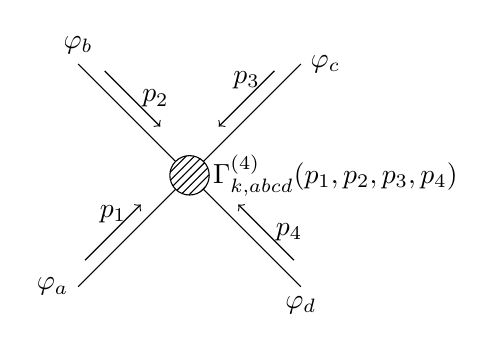
\begin{tikzpicture}[rotate=45]
  \draw (-2,0) node[left] {$\varphi_a$} -- (2,0) node[right] {$\varphi_c$} (0,2) node[above] {$\varphi_b$} -- (0,-2) node[below] {$\varphi_d$};
  \draw[->,yshift=5pt] (-1.7,0) -- (-0.7,0) node[midway,above] {$p_1$};
  \draw[<-,yshift=5pt] (0.7,0) -- (1.7,0) node[midway,above] {$p_3$};
  \draw[->,xshift=5pt] (0,1.7) -- (0,0.7) node[midway,right] {$p_2$};
  \draw[<-,xshift=5pt] (0,-0.7) -- (0,-1.7) node[midway,right] {$p_4$};
  \draw[fill=white,postaction={pattern=north east lines}] (0,0) circle (0.25) node[right=5pt] {$\Gamma_{k,abcd}^{(4)}(p_1,p_2,p_3,p_4)$};
\end{tikzpicture}
\end{document}